%!TEX encoding = UTF-8 Unicode
%!TEX root = ../lect-week13.tex

%%%

\ifkompendium\else

\Subsection{Repetition, uppsamling, kursutvärdering}

\begin{Slide}{Repetition}
  \begin{itemize}
    \item Fortsättning på extenta-genomgång
    \item Grumligtlådan
    \item Nyfiken-på-lådan
  \end{itemize}
\end{Slide}


\begin{Slide}{Uppsamling: obligatoriska moment}\SlideFontSmall
\begin{itemize}
\item Kolla vilka oblikatoriska moment du har kvar här:
\url{http://cs.lth.se/pgk/sam}
\item Sök på din födelsemånad/dag, tex 0102 för andra januari.
\item Du måste ha gjort \Emph{kontrollskrivning} och vara godkänd på alla \Emph{laborationer} (utom rekommenderade men valfria w12\_survey) och vara godkänd på \Emph{projektet} för att få tentera \code{pgk}!
\item Din ev. \Emph{samarbetsbonus} (max 5p) från kontrollskrivningen gäller endast första ordinarie tentamenstillfälle.
\item Läs \Alert{alla} instruktioner \Alert{noga} och \Alert{anmäl dig} här: \\
\href{http://www.student.lth.se/studieinformation/anonyma-tentor/}{www.student.lth.se/studieinformation/anonyma-tentor}
\item Du måste vara \Emph{godkänd} på alla obligatoriska labbar och projektet \Alert{innan du får påbörja pfk} \href{http://cs.lth.se/edaa01vt}{EDAA01}
\item Använd återstående \Emph{resurstider} för \Alert{redovisning av labbar/projekt}.
\end{itemize}
\end{Slide}

\begin{Slide}{CEQ -- Course Experience Questionnaire}\SlideFontSmall
\begin{itemize}
\item Görs på hela LTH på samma sätt. Alla får länkar via mejl.
\item Snälla fyll i CEQ! Jag är \Alert{mycket tacksam} för all konstruktiv feedback! \\ Hög svarsfrekvens är viktigt för att kunna dra slutsatser om variationen i svaren och signifikansen i sammanställningen.
\item Del 1: Generella påståenden, alla med 5-gradig skala: \\ tar helt avstånd ... instämmer helt
\item Del 2: \Emph{Fritextfrågor}: \\
''Vad  tycker  du  var  det  bästa  med  den här  kursen?'' \\
''Vad  tycker  du  främst  behöver  förbättras?''
\item Mer om CEQ här: \url{https://www.ceq.lth.se/}
\item \Emph{Fördel} med CEQ: Samma alla kurser alla år medger jämförelse över tid.
\item \Alert{Begränsning}: Saknar frågor kopplat till specifika kursmoment.
\end{itemize}
\end{Slide}

\begin{Slide}{Kursspecifik utvärdering om specifika kursmoment}\SlideFontSmall
\begin{itemize}
\item Jag vill gärna att \Alert{alla} gör den LTH-gemensamma, anonyma kursutvärderingsenkäten \href{https://www.ceq.lth.se/}{CEQ}. Dina fritext-kommentarer om vad som är det bästa med kursen och vad som främst behöver förbättra emottages mycket tacksamt i CEQ-utvärderingen!
\item Jag kommer att komplettera CEQ med en \Emph{kursspecifik utvärdering} av specifika kursmoment i denna kurs och jag är därför \Alert{mycket tacksam} om alla fyller enkäten när länk kommer via mejl.
\item Jag behandlar dina svar \Alert{konfidentiellt}, men sparar din email så att jag kan återkomma om jag mot förmodan undrar något mer.
\item Din input är \Emph{mycket värdefull} vid framtida kursutveckling!
\end{itemize}
\end{Slide}

\begin{Slide}{Intresserad av att arbeta som handledare?}
\begin{itemize}
\item Vi har ständigt behov av nya handledare i våra kurser
\item Det är lärorikt att jobba som timanställd handledare
\item Kontakta \verb|bjorn.regnell@cs.lth.se| eller annan kursansvarig i den kurs du vill jobba
\end{itemize}
\end{Slide}

\Subsection{Utblick: Vad kan framtidens dataingenjörer från LTH?}

\begin{Slide}{Framtidens (data)ingenjör}
Vårt utbildninguppdrag vid institutionen för Datavetenskap:
\begin{itemize}
  \item Utbilda \Emph{dataingenjörer} för \Alert{framtidens} arbetsmarknad
  \item Säkerställa att alla typer av LTH-ingenjörer har \Emph{tillräckliga} kunskaper i datavetenskap och modern systemutveckling
  \item Förbereda för \Emph{livslångt lärande} inom \Alert{datavetenskap}: rätt grundkunskaper för att kunna lära sig ny teknik/forskning
  \item Tillgodo se behovet av den \Emph{djupa datavetenskapliga kompetens} som dagens och morgondagens näringsliv är i så \Alert{skriande behov} av: \\
  \url{https://computersweden.idg.se/2.2683/1.693037/bransch-it-jobb} \\
\end{itemize}
\Alert{''Nytt branschlarm: Behövs 70000 fler som jobbar med it''}
\end{Slide}

\begin{Slide}{Vad är de två allra största utmaningarna för framtiden inom software engineering?}
  \begin{enumerate}
    \item Kompetensbristen
    \item
    \pause Att hantera den ständigt ökande \Alert{komplexiteten}
  \end{enumerate}
  \pause(Del)lösning: \pause \Emph{kraftfullare abstraktionsmekanismer}
\end{Slide}


\begin{Slide}{Framtidens kurser för D-are}
\begin{itemize}
  \item \href{http://cs.lth.se/utbildning/}{Undervisningen i Datavetenskap} har fördubblats på 5 år
  \item D-programmet utvecklas: flera nya kurser införda/på gång
  \item Exempel på kurser som direkt bygger på grundkursen i programmering med Scala, \code{pgk}:
\begin{itemize}
\item Fördjupningskursen (Java)
\item \Alert{Ny sedan 2016:} Utvärdering av programvarusystem (R)
\item \Alert{Ny sedan 2016:} Diskreta strukturer (Clojure)
\item Programvaruutveckling i grupp (Java)
\item Objekt-orienterad modellering och design (Java)
\item \Alert{Numera obligatorisk:} Funktionsprogrammering (Haskell)
\end{itemize}
\item Exempel på pågående/föreslagen kursutveckling:
\begin{itemize}
  \item Machine Learning
  \item Concurrency, distribution, real-time embedded systems
  \item Open Source Software Engineering
  \item Development for web apps, cloud, back-end, (front-end)
  \item Tool chain for continuous software engineering
\end{itemize}
\end{itemize}
\end{Slide}


\begin{Slide}{Mål med nya grundkursen i Scala}
\begin{itemize}
  \item Hantera stora spridningen i förkunskaper. Andel nybörjare:
  \begin{itemize}
    \item 2015: ca 20\% har aldrig kodat före kursstart
    \item 2016: ca 30\% har aldrig kodat före kursstart
    \item 2017: ca 40\% har aldrig kodat före kursstart
  \end{itemize}
  \item Hantera stora spridningen i förmåga att ta sig över trösklar:
  \begin{itemize}
    \item Många studenter har höga ambition och hög motivation
    \item Några studenter har stora svårigheter i början
  \end{itemize}
  \item Modernisera innehåll och pedagogik:
  \begin{itemize}
    \item grundläggande objektfunktionell programmering
    \item använda ett modernt, kraftfullt samlingsbibliotek
    \item oföränderliga datastrukturer
    \item samarbete mellan studenter
    \item allt kursmaterial är fri öppenkällkod med studentdeltagande i den kontinuerliga utvecklingen:
    \url{https://github.com/lunduniversity/introprog}
  \end{itemize}
\end{itemize}
\end{Slide}


\begin{Slide}{Varför Scala?}
Lätt för nybörjare och intressant för icke-nybörjare:
\begin{itemize}
\item enhetlig semantik; alla värden är objekt
\item koncis och uttrycksfull semantik
\item interaktivt lärande med Scala REPL
\item Multi-paradigm, pragmatiskt: \\ imperativt, objekt-orienterat, funktionellt
\item Rik semantik: kan demonstrera många koncept
\item Modernt språk som utvecklas med forskningen
\item Språket och verktygen är fri öppen källkod
\end{itemize}
\pause Några risker som vi identifierade som inte visat sig vara några problem: omogna verktyg, brist på kursmaterial för nybörjare, kritisk massa i communityn, industriell spridning.
%\begin{itemize}\fontsize{9}{10}\selectfont
%\item Tools not becoming mature fast enough?
%\item Lack of beginner-oriented teaching material?
%\item Future industrial relevance?
%\item Critical mass of community?
%\end{itemize}
\end{Slide}


\Subsection{Utblick: Framtiden för Scala?}

\begin{Slide}{Hur populärt blir Scala bland utvecklare i framtiden?}
Mest älskade språk på \code{stackoverflow} (2016)
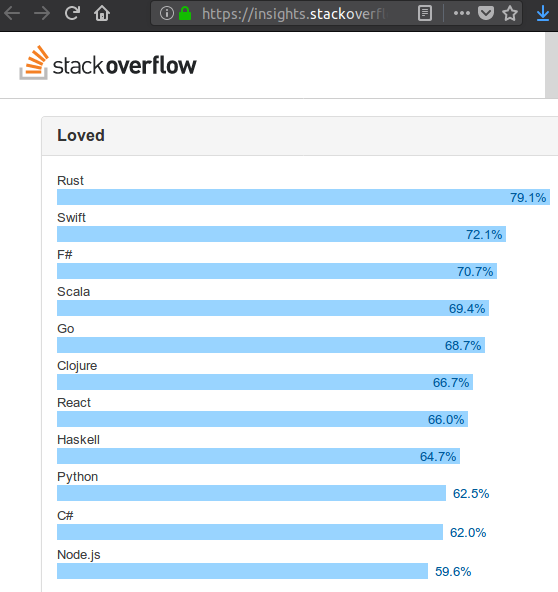
\includegraphics[width=0.9\textwidth]{../img/w14/most-loved-2016.png}
\end{Slide}

\begin{Slide}{Hur ser framtidens jobbmarknad för Scala ut?}\SlideFontTiny

\hspace{-2.5em}\begin{minipage}{1.0\textwidth}
Jobbmarknaden för Scala växer globalt och i Sverige:

\begin{minipage}{0.48\textwidth}
\href{www.indeed.com/joptrends/q-scala.html}{www.indeed.com/joptrends/q-scala.html}\\
\vspace{1em}
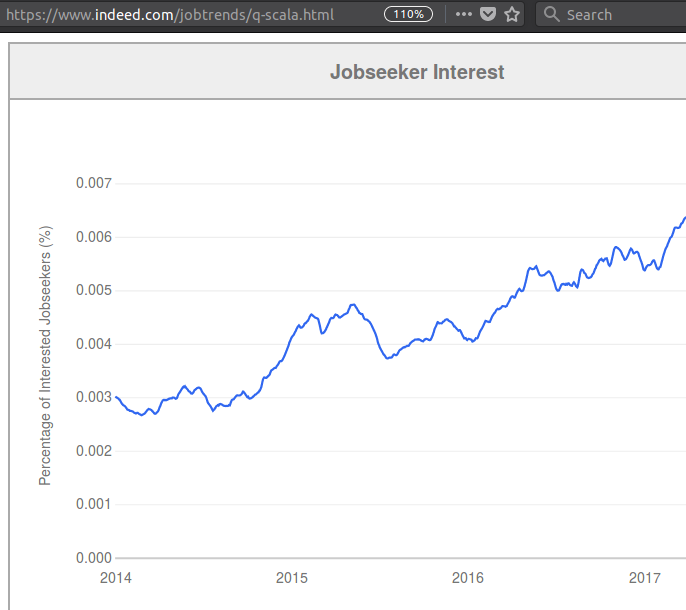
\includegraphics[width=1.0\textwidth]{../img/w14/scala-jobs-indeed-2017.png}~~
\end{minipage}
\hfill\begin{minipage}{0.48\textwidth}
\vspace{1.25em}
\href{https://www.linkedin.com/jobs/search/?keywords=scala&location=Sweden&locationId=se%3A0}{https://www.linkedin.com/jobs/search/?keywords=scala}\\
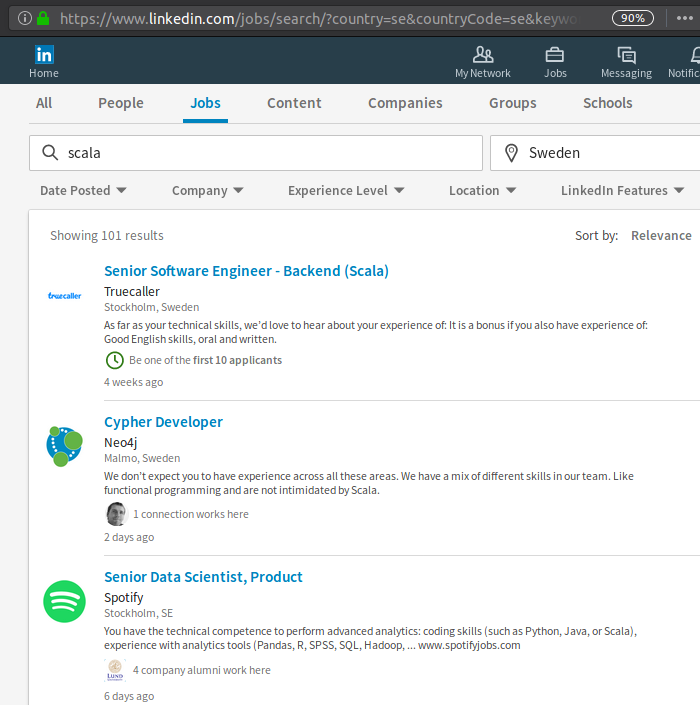
\includegraphics[width=1.2\textwidth]{../img/w14/scala-jobs-sweden-linkedin-2017-dec07.png}
\end{minipage}
\end{minipage}
\end{Slide}


\begin{Slide}{Hur ser framtiden ut för Scala?}\SlideFontSmall

Framtiden för \Emph{Scala}:
\begin{itemize}
\item Scala 2.12 bättre bytekod med lambda i JVM Java 8
\item Scala 2.13 bättre standardbibliotek
\item Ny kompilator: \Emph{dotty}; Nytt format ''över'' bytekod: \Emph{Tasty}
\item Scala.JS: dela kod+kompetens mellan backend och frontend
\item Scala native: kör Scala kompilerat direkt ''på metallen''
\item Scala-ramverk för stordata, massiv parallellism, AI, ...
\end{itemize}
\end{Slide}

\Subsection{Överraskning: LUFOSS}
\begin{Slide}{LUFOSS: Lund University Fund for Open Source Software}
\begin{itemize}
  \item Prisutdelning
  \begin{itemize}
    \item Studentpris
    \item Doktorandpris
    \item Hederspris
  \end{itemize}
  \item Gästföreläsning hederspristagare
\end{itemize}
\end{Slide}


\Subsection{Avslutning}

\begin{Slide}{Hoppas att pgk-kursen varit intressant och lärorik!}
\pause
\includegraphics[width=5cm]{../img/gurka.jpg}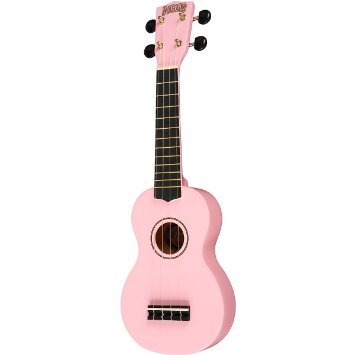
\includegraphics[width=5cm]{../img/ukulele.jpg}
\end{Slide}

\begin{Slide}{Ett stort TACK...}
\begin{itemize}
  \item
... till alla \Emph{handledare} som jobbat hårt för att ni ska lära er så mycket som möjligt!
\item ... till alla \Alert{studenter} som gått kursen för:
\begin{itemize}
\item ... att ni kämpat så hårt!
\item ... att ni ställt massor med frågor!
\item ... att det har varit så hög närvaro på föreläsningarna!
\item ... att ni hjälp till med värdefull återkoppling!
\item ... att ni är så konstruktiva och verkligen vill lära er!
\end{itemize}
\vspace{2em} \pause

\end{itemize}
\Alert{Ett stort LYCKA TILL på vägen till att bli en \\ kompetent och innovativ systemutvecklare!}
\end{Slide}



\fi
